\documentclass[a4paper]{article}

\usepackage[french]{babel}
\usepackage[T1]{fontenc}
\usepackage[utf8]{inputenc}
\usepackage{amsmath}
\usepackage{graphicx}
\usepackage{lmodern}
\usepackage[left=3cm, right=3cm, bottom=4cm, top=4cm]{geometry}
\usepackage{array}
\usepackage{pdfpages}
\usepackage{listings}
\usepackage{algorithm}
\usepackage{algorithmic}
\usepackage{sidecap}
\usepackage{pdflscape}
\usepackage{hyperref}
\usepackage{tipa}
\usepackage{multirow}
\usepackage[gen]{eurosym}
\usepackage{float}
\DeclareUnicodeCharacter{20AC}{\euro{}}

\usepackage{hyperref}
\hypersetup{    
    colorlinks,
    citecolor=black,
    filecolor=black,
    linkcolor=black,
    urlcolor=black
}

\title{Bilan de planification}

\author
{
    Pierre-Marie {\sc Airiau}\\
    Valentin {\sc Esmieu}\\
    Maud {\sc Leray}\\
    %Hoel {\sc Kervadec}\\
    %Florent {\sc Mallard}\\
    %Corentin {\sc Nicole}\\
    %ON VOUS AIME LES COPAINS
}

\date{\today}

\newcommand{\pagevierge}[0]{\newpage\thispagestyle{empty}\null\newpage}
\newcommand{\glasir}[0]{Glasir}
\newcommand{\ttable}[0]{{\sc Table}}
\newcommand{\ffigure}[0]{{\sc Figure}}

\newcommand{\nomRepart}[1]{\multicolumn{2}{c||}{\textbf{#1}}}
\newcommand{\nomRepartt}[1]{\multicolumn{2}{c|}{\textbf{#1}}}

\begin{document}
    % Ouh c'est sale.
    \hypersetup{pageanchor=false}
    
\includepdf[pages=1]{figure/couv.pdf}
    \hypersetup{pageanchor=true}
    
    \newpage
    \thispagestyle{empty}
    \mbox{}
    
    \newpage
    
    \setcounter{tocdepth}{2}
    \tableofcontents
    \setlength{\parskip}{10pt}
    
    \newpage
    \thispagestyle{empty}
    \mbox{}

    \newpage
    \section{Introduction}

rappel énoncé/problématique

réponse à la pb

    \newpage
    \section{Planification initale}
\label{sec:planifInit}

Cette section a pour but de rappeler les grandes lignes de la planification initiale du projet, qui avait été détaillée dans le rapport de planification~\cite{planif}. Pour rappel, la méthode de gestion de projet que nous avons choisie d'appliquer est la méthode SCRUM, dont le principe est brièvement rappelé dans la {\sc sous-section}~\ref{ssec:scrum}.

\subsection{La méthode SCRUM}
\label{ssec:scrum}

En décembre dernier, après avoir déjà rédigé et rendu les rapports de pré-étude~\cite{pre_etude} et de spécifications fonctionnelles~\cite{spec_fonc}, il a fallu penser à la planification du développement de Glasir. Après discussions, nous nous sommes finalement dirigés vers une méthode agile proche du \og \textsc{Scrum} \fg{}. Ce choix s'est basé sur les constats suivants :

Depuis le début du projet, un \og coordinateur \fg{} était responsable de la réalisation et du rendu d'un livrable (rapport, version logicielle, etc). Ce rôle, attribué à une nouvelle personne à chaque nouveau livrable, était assimilable au rôle de \og Scrum Master \fg{} tel que défini dans la méthode \textsc{scrum}.

Le coordinateur endossait également la responsabilité de \og Product Owner \fg{}, partagée avec les encadrants du projet pour ce qui est de la définition des objectifs et surtout de l'acceptation des livrables.

Au lieu de la mêlée quotidienne du \textsc{Scrum}, un rythme hebdomadaire a été adopté pour les réunions car Glasir n'est pas un projet à temps plein. 

Enfin, le développement de chaque version a été divisé en sprints au cours desquels chaque développeur était associé à un sous-ensemble de tâches nécessaires à la réalisation de Glasir. Ces tâches ont constituées les \og Users Stories \fg{} du projet, et sont détaillées dans la \textsc{sous-section}~\ref{ssec:repartition}. Avant de revenir sur cette répartition, quelques rappels sur le versionnement de l'implémentation s'imposent dans la {\sc sous-section}~\ref{ssec:versions}.

\subsection{Versionnement du développement}
\label{ssec:versions}

L'implémentation de Glasir (et des améliorations apportées à ADTool en parallèle) a été séparée en trois versions (deux intermédiaires et une finale), chacune étant concrétisée par un rendu aux encadrants sous la forme d'un exécutable fonctionnel. Le contenu de ces trois livrables est rapidement décrit ci-dessous.

\paragraph{Version 0.1} Huit grandes tâches ont été identifiées pour cette version et sont présentées dans la {\sc Table} \ref{tab:taches_units_1}. 
            \begin{table}[H]
                \centering
                \begin{tabular}{|c|r|l|c|r|}
                    \hline
                    \textbf{Cible} & \textbf{Id} & \textbf{Tâche} & \textbf{Technologies} & \textbf{Durée}\\
                    \hline

                    \multirow{5}{*}{\glasir{}} & 1.1 & Squelette interface & WPF & 6h\\
                    \cline{2-5}
                     & 1.2 & Gestion fichiers projet & C++ & 20h\\
                    \cline{2-5}
                     & 1.3 & Intégration ADTool dans \glasir & JNI & 20h\\
                    \cline{2-5}
                     & 1.4 & \'Evaluateur de fonction & Java & 12h\\
                    \cline{2-5}
                     & 1.5 & Interface évaluateur & WPF & 8h\\
                    \hline

                    \multirow{3}{*}{ADTool} & 1.6 & Valuation ADTrees & \multirow{3}{*}{Java} & 18h\\
                    \cline{2-3} \cline{5-5}
                     & 1.7 & Refonte langage des ADTrees & & 16h\\
                    \cline{2-3} \cline{5-5}
                     & 1.8 & Vue globale des paramètres & & 12h\\
                    \hline

                    \multicolumn{4}{|l|}{\bf Total} & {\bf 112h}\\
                    \hline
                \end{tabular}
                \caption{Tâches associées au développement de \glasir{} version 0.1.}
                \label{tab:taches_units_1}
            \end{table}

\paragraph{Version 0.2} Le développement de la version 0.2 est découpé en cinq tâches, résumées dans la {\sc table} \ref{tab:taches_units_2}.
            \begin{table}[h]
                \centering
                \begin{tabular}{|c|r|l|c|r|}
                    \hline
                    \textbf{Cible} & \textbf{Id} & \textbf{Tâche} & \textbf{Technologies} & \textbf{Durée}\\
                    \hline

                    \multirow{4}{*}{\glasir{}} & 2.1 & Algorithme filtrage & C++ & 24h\\
                    \cline{2-5}
                     & 2.2 & Interface filtre & WPF & 15h\\
                    \cline{2-5}
                     & 2.3 & Multiples instances d'ADTool & C++, WPF & 20h\\
                    \cline{2-5}
                     & 2.4 & Affichage arbre filtré & Java, WPF & 16h\\
                    \hline

                    \multirow{1}{*}{ADTool} & 2.5 & Couper/copier/coller & \multirow{1}{*}{Java} & 25h\\
                    \hline

                    \multicolumn{4}{|l|}{\bf Total} & {\bf 100h}\\
                    \hline
                \end{tabular}
                \caption{Tâches associées au développement de \glasir{} version 0.2.}
                \label{tab:taches_units_2}
            \end{table}

\paragraph{Version 1.0} Quatre tâches ont été identifiées pour la version 1.0 de \glasir{}, présentées dans la {\sc Table} \ref{tab:taches_units_3}.
            \begin{table}[h]
                \centering
                \begin{tabular}{|c|r|l|c|r|}
                    \hline
                    \textbf{Cible} & \textbf{Id} & \textbf{Tâche} & \textbf{Technologies} & \textbf{Durée}\\
                    \hline

                    \multirow{4}{*}{\glasir{}} & 3.1 & Optimiseur & C++, WPF & 30h\\
                    \cline{2-5}
                     & 3.2 & Bibliothèque de modèles & C++, WPF & 20h\\
                    \cline{2-5}
                     & 3.3 & Harmonisation interface & WPF & 16h\\
                    \cline{2-5}
                     & 3.4 & Packaging & - & 8h\\
                    \hline

                    \multirow{1}{*}{ADTool} & 3.5 & Ctrl-Z & \multirow{1}{*}{Java} & 16h\\
                    \hline

                    \multicolumn{4}{|l|}{\bf Total} & {\bf 90h}\\
                    \hline
                \end{tabular}
                \caption{Tâches associées au développement de \glasir{} version 1.0.}
                \label{tab:taches_units_3}
            \end{table}

À l'issue de cette première division du travail à réaliser, il a fallu répartir entre les développeurs les tâches citées précédemment pour chacune des versions. Ces assignations sont rappelées dans la {\sc sous-section}~\ref{ssec:repartition}.

\subsection{Répartition des tâches}
\label{ssec:repartition}

Pour répartir correctement les tâches unitaires présentées dans la {\sc sous-section}~\ref{ssec:versions}, nous avons fait le choix de \og spécialiser \fg{} chacun des trois développeurs comme indiqué ci-après :

\begin{itemize}
\item Pierre-Marie {\sc Airiau} était en charge des trois modules principaux de Glasir et des principaux problèmes algorithmiques ;
\item Valentin {\sc Esmieu} s'occupait surtout de l'interface de Glasir et de son fonctionnement global ;
\item Maud {\sc Leray} était responsable des améliorations apportées à ADTool.
\end{itemize}

Ce choix de planification permettait non seulement d'équilibrer le nombre d'heures de travail par personne, mais aussi de limiter pour chacun l'apprentissage de nouvelles technologies, ce qui aurait sinon entraîné un ralentissement dans l'avancement du projet. La répartition exacte des tâches est définie dans la {\sc table}~\ref{tab:repartition}.

\begin{table}[H]
            \centering
            \begin{tabular}{|l|c|r||c|r||c|r|}
                \hline
                \multirow{2}{*}{} & \nomRepart{Pierre-Marie A.} & \nomRepart{Valentin E.} & \nomRepartt{Maud L.}\\
                \cline{2-7}
                 & {\bf Id tâche} & {\bf Durée} & {\bf Id tâche} & {\bf Durée} & {\bf Id tâche} & {\bf Durée}\\
                \hline
                {\bf Version 0.1} & - & {\bf 38h} & - & {\bf 34h} & - & {\bf 40h}\\
                 & 1.3 & 10h & 1.1 & 6h & 1.2 & 10h\\
                 & 1.4 & 12h & 1.2 & 10h & 1.6 & 18h\\
                 & 1.7 & 16h & 1.3 & 10h & 1.8 & 12h\\
                 & - & - & 1.5 & 8h & - & -\\
                \hline
                {\bf Version 0.2} & - & {\bf 39h} & - & {\bf 33h} & - & {\bf 28h}\\
                 & 2.1 & 24h & 2.3 & 20h & 2.4 & 16h\\
                 & 2.2 & 15h & 2.5 & 13h & 2.5 & 12h\\
                \hline
                {\bf Version 1.0} & - & {\bf 25h} & - & {\bf 23h} & - & {\bf 42h}\\
                 & 3.1 & 15h & 3.1 & 15h & 3.2 & 10h\\
                 & 3.2 & 10h & 3.4 & 8h & 3.3 & 16h\\
                 & - & - & - & - & 3.5 & 16h\\
                \hline
                {\bf Total} & \multicolumn{2}{r||}{{\bf 102h}} & \multicolumn{2}{r||}{{\bf 100h}} & \multicolumn{2}{r|}{{\bf 110h}}\\
                \hline
            \end{tabular}
            \caption{Répartition des tâches, par personne et par version.}
            \label{tab:repartition}
        \end{table}

Ici s'arrête le résumé de la planification initiale, il est donc temps de passer à la comparaison de cette dernière avec la planification effective constatée à l'issue du développement de Glasir. C'est le but de la {\sc Section}~\ref{sec:ecarts}. 

    \newpage
    \section{Écarts à la planification}


Abandon multi-params

Avance

Retour sur fonctionnalités précedentes (editeur fonctions)

Communication glasir-adtool : View-mode

Support du multi ctrl Z

ameliorations mineures sur adtool (nommage des fenetres, ...)

    \newpage
    \section{Ergonomie du logiciel}
	Des fonctionnalités plus secondaires seront implémentées dans le but de rendre \glasir{} suffisamment ergonomique pour être utilisé avec confort. Ces fonctionnalités n'apporteront pas de nouveautés en terme d'analyse, mais permettront de faciliter la manipulation des arbres dans ADTool et de rendre \glasir{} simple d'utilisation.	

	\subsection{Ouverture simultanée de plusieurs arbres}
		Dans sa version actuelle, ADTool ne permet de travailler que sur un seul arbre à la fois. Cette limitation est assez handicapante : par exemple, l'utilisateur ne peut pas ouvrir deux arbres en même temps pour les comparer. \glasir{} permettra donc d'ouvrir plusieurs instances d'ADTool, chacune contenant un arbre. Ces différentes instances se regrouperont sous la forme d'onglets situés dans l'interface de \glasir{}.
	
	\subsection{Hiérarchie des arbres}
		L'ouverture simultanée de plusieurs arbres induit la possibilité de manipuler un grand nombre d'arbres dans le cadre d'un même projet. Dans le but d'aider l'utilisateur à organiser facilement son projet, \glasir{} fournira dans un dock latéral, une arborescence de dossiers et de sous-dossiers contenant les différents arbres utilisés.

	\subsection{Bibliothèque de modèles}
		Il n'est pas forcément facile pour l'utilisateur de créer un arbre à partir de rien. C'est pourquoi \glasir{} fournira une bibliothèque d'arbres génériques, aidant ainsi l'expert à démarrer son projet. Cette bibliothèque de modèles sera dupliquée pour être propre à chaque nouveau projet, permettant ainsi à l'utilisateur de modifier, compléter ou élaguer les arbres selon ses besoins. Notre étude portant sur le réseau STAR, la bibliothèque de modèles génériques intégrera principalement des ADTrees relatifs aux réseaux de transport en commun rennais. 

		
		Si l'utilisateur construit un nouvel arbre qu'il juge pertinent de réutiliser dans un autre projet, il pourra enregistrer cet arbre comme nouveau modèle, qui se rajoutera donc à la bibliothèque. \glasir{} verra ainsi sa bibliothèque de modèles s'étoffer progressivement au cours du temps.


	
	\subsection{Couper/copier/coller}	
		Actuellement, ADTool ne permet pas l'utilisation des fonctions \emph{couper}/\emph{copier}/\emph{coller}, qui pourraient pourtant s'avérer pratiques lors de la création d'un arbre. Par exemple, dans le cas de l'oubli d'un nœud père, l'instauration de ces fonctionnalités permettrait de déplacer facilement les fils concernés de l'ancien nœud père vers le nouveau.
		
		En conséquence, nous allons modifier ADTool pour qu'il implémente ces fonctionnalités. Ainsi, la sélection d'un nœud entraînera la sélection de ses fils, afin de pouvoir couper ou copier ces nœuds facilement. Les raccourcis clavier \og classiques \fg{}  de ces fonctions (\emph{CTRL+X, CTRL+C, CTRL+V}) seront mis en place.


	\subsection{Amélioration du codage des arbres}
		ADTool affiche actuellement dans son interface une section nommée \emph{ADTerm Edit}. Celle-ci contient une représentation de l'arbre sous un format texte, en utilisant un langage propre au logiciel. Lors de la modification de l'arbre dans l'éditeur graphique, ADTool met à jour le texte correspondant en temps réel et de manière automatique. L'inverse est également vrai : il est possible de changer les labels des nœuds, ou les opérateurs, directement depuis \emph{ADTerm Edit} afin d'afficher ensuite le résultat graphiquement.

		Mais le langage qui permet de décrire les arbres sous format texte n'est pas très lisible : il ne contient par exemple pas le nom des nœuds autres que les feuilles. Sur la {\sc Figure} \ref{fig:int_adTool}, on peut constater que le code indique le nom des deux feuilles \og Acheter le matériel nécessaire \fg{} et \og Essayer les clés possibles \fg{}, et que la conjonction est bien précisée par l'opérateur \og ap \fg{} (\og op \fg{} en cas de disjonction). Mais aucune référence n'est faite au label du nœud père \og Casser le chiffrage \fg{}. Nous modifierons la grammaire pour corriger ce défaut, afin de rendre l'utilisation de cette fenêtre plus intuitive.

		\begin{figure}[h]
			\centering
			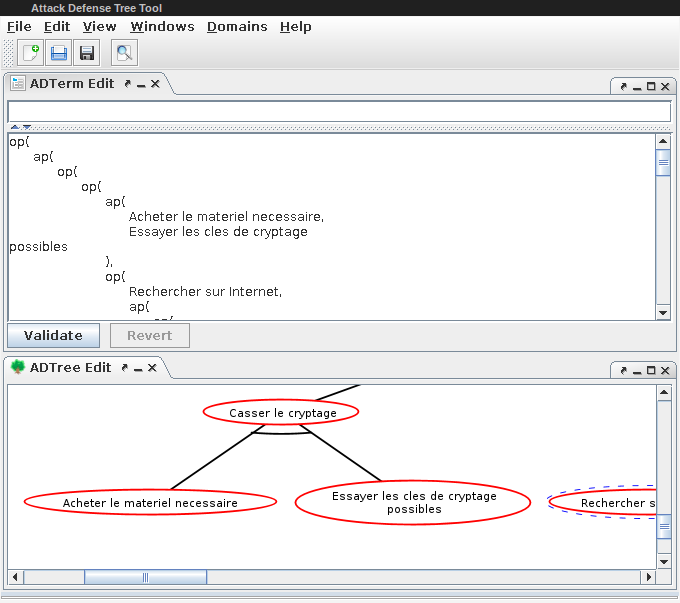
\includegraphics[width=0.6\textwidth]{figure/interface_adtool.png}
			\caption{L'interface d'ADTool. En haut, l'arbre au format texte ; en bas, sa représentation graphique.}
			\label{fig:int_adTool}
		\end{figure}
	
	\subsection{Annulation d'une action}	
		Pour le moment, effectuer une action sous ADTool est irréversible. Cela n'est pas grave pour certaines actions rapides à effectuer, telles que le renommage d'un nœud. Mais supprimer un nœud (ce qui implique la disparition de tous ses nœuds fils s'il y en a) par erreur peut entraîner un travail énorme, et donc une perte de temps. La possibilité de revenir à l'état précédent de l'arbre (par le raccourci clavier classique \emph{CTRL+Z}) éviterait d'avoir à refaire ce travail de construction fastidieux. Nous souhaitons créer au moins une sauvegarde de l'état précédent, afin de pouvoir annuler la dernière modification effectuée. Si possible, nous envisageons l'implémentation d'une pile circulaire contenant les N derniers états (chaque modification entraînant la création d'un nouvel état) avec un curseur pointant sur l'état courant. Cela permettrait de revenir en arrière sans contraintes. 

		Cette fonctionnalité sera implémentée en utilisant le patron de conception \emph{Commande}. Les actions de l'utilisateur dans ADTool seront sauvegardées pour pouvoir, quand l'utilisateur demandera l'annulation de son action, effectuer l'action inverse. 

	\subsection{Vue globale des paramètres}
		Dans l'état actuel d'ADTool, lorsqu'un arbre est valué, un seul paramètre est affiché (le même pour tous les nœuds) même si plusieurs paramètres sont utilisés en réalité. En effet, chaque valuation a un onglet propre, dans lequel elle est la seule effectivement affichée sur l'arbre. Nous souhaitons créer un onglet plus général, dans lequel tous les paramètres voulus peuvent être visibles sur l'arbre en simultané. C'est ensuite à l'expert de décider des paramètres qu'il juge utile d'afficher. Cela serait aussi valable pour les paramètres de synthèse évoqués dans la {\sc Sous-section} \ref{subsection:synthese}.
	
		Pour une meilleure lisibilité, chaque paramètre aura une couleur différente, et l'arbre sera accompagné d'une légende résumant ce jeu de coloration et ses correspondances. Nous devrons également gérer la taille des nœuds, pour que les paramètres ne dépassent pas de la bulle. Un tel système étant déjà présent dans ADTool pour gérer les labels, il suffira de l'étendre à l'affichage des paramètres.

		Maintenant que les différentes fonctionnalités à développé ont été défini, une première planification peut être présentée. 

    \newpage
    \section{Conclusion}

    \newpage

    \bibliographystyle{plain}
    \bibliography{input/biblio}

    % Manoucherie incoming
    \pagevierge
    \ifthenelse{\isodd{\thepage}}
    {\pagevierge}
    {}
    
\includepdf[pages=2]{figure/couv.pdf}
\end{document}
